This section builds on the classification results presented earlier. The motivation for classification is to better understand underlying traffic patterns before performing forecasting. By separating network sites into seasonal and non-seasonal groups, it becomes possible to evaluate whether different traffic dynamics require different forecasting strategies. \\

All forecasting models are evaluated using a chronological 80/20 train-test split. The first 80\% of each time series is used for training, while the final 20\% is reserved for testing. This split preserves temporal order and avoids information leakage from future observations. The test set is used as the common validation set across all models. \\

\textbf{Root Mean Squared Error (RMSE)} \\
Model performance is evaluated using the Root Mean Squared Error (RMSE), defined as:

\begin{equation}
	\text{RMSE} = \sqrt{\frac{1}{n} \sum_{i=1}^{n} (y_i - \hat{y}_i)^2}
	\label{eq:rmse}
\end{equation}

where $y_i$ is the observed value and $\hat{y}_i$ is the predicted value. RMSE penalizes larger errors more heavily than absolute error due to the squaring term, while remaining in the same unit as the target variable. This makes it suitable for network traffic forecasting, where large underestimations of peak load can lead to capacity issues. \\

\subsection{Baseline Models}

Before introducing more complex forecasting approaches, several baseline models are defined to provide reference performance levels \cite{forecasting_book}.  These baselines allow for a fair evaluation of whether more advanced methods provide meaningful improvements. \\

The dataset is evaluated under three settings, seasonal cells, non-seasonal cells, and a combined dataset. This enables analysis of whether traffic behavior differs across network environments. The cells were split into the different groups by the t-test as shown in figure \ref{eq:ttest}, if the p-value was below 0.05, there was not enough evidence that the cell was seasonal and it was put in the non-seasonal category.  \\

The forecasting target is the daily peak traffic volume, defined as the maximum observed hourly traffic within a day as seen in figure \ref{fig:U1_vs_R1_daily_max}. This metric is particularly important for network planning, as it reflects peak load conditions that are critical for capacity management. \\

\begin{table}[h]
	\centering
	\begin{tabular}{lccc}
		\hline
		\textbf{Model} & \textbf{Seasonal RMSE} & \textbf{Non-Seasonal RMSE} & \textbf{Overall RMSE} \\
		\hline
		Seasonal Naive & 2.36 & 2.58 & 2.51 \\
		Mean Naive     & 1.77 & 1.99 & 1.92 \\
		Previous Naive & 1.85 & 1.97 & 2.51 \\
		\hline
	\end{tabular}
	\caption{RMSE obtained by the baseline forecasting models using the 80/20 chronological train-test split. Lower values indicate better forecasting performance.}
	\label{tab:baseline_models}
\end{table}

Table~\ref{tab:baseline_models} presents the baseline model results. The seasonal naive model, which forecasts each period by repeating the corresponding values from the previous year, performs worst across all splits. This suggests that traffic patterns are not stable year over year. \\

The mean naive model forecasts using the training set mean, while the previous naive model uses the most recently observed value as the prediction. A notable pattern is seen when comparing the two across dataset splits, the mean model performs better on non-seasonal cells, while the previous value model performs better on seasonal cells. This is consistent with the underlying traffic patterns, non-seasonal cells shows relatively stable behavior over time, making the mean a reliable predictor, whereas seasonal cells are subject to gradual trends and periodic fluctuations, meaning recent observations carry more predictive information than the historical average. \\

It should be noted that MSE values are not directly comparable across dataset splits, as seasonal and non-seasonal cells differ in their underlying traffic variance. Comparisons are therefore made within each group independently. \\

\subsection{ARIMA}
ARIMA (AutoRegressive Integrated Moving Average) is a widely used statistical model for forecasting time series data. It is designed to capture patterns such as autocorrelation and trends in the data.

The model is defined by three parameters: $p$, $d$, and $q$.
\begin{itemize}
    \item $p$: the number of autoregressive (AR) terms, which model the relationship between the current value and its past values.
    \item $d$: the degree of differencing used to make the series stationary.
    \item $q$: the number of moving average (MA) terms, which model the relationship between the current value and past forecast errors.
\end{itemize}

A seasonal extension $(P, D, Q, m)$ can also be included, where $m$ represents the number of time steps in one seasonal cycle. This allows the model to capture repeating patterns that occur every $m$ periods. \\

The optimal parameters are selected by minimizing the Akaike Information Criterion (AIC), which balances model fit and complexity. \\

\subsubsection{SARIMAX}
SARIMAX is an extension of the ARIMA model. The \textit{S} represents the seasonal component introduced previously, while the \textit{X} indicates the inclusion of exogenous input features. Unlike ARIMA, which only models the historical behavior of the time series itself, SARIMAX can additionally incorporate external variables that may influence the forecasting.

\subsubsection{Model Optimization}

The following method was used to validate the ARIMA forecasting approach on the dataset. As described earlier, the data consists of two groups seasonal and non-seasonal. For each individual cell time series, the auto ARIMA function [Put python documentaration link here]  was applied to determine the parameter set that minimizes the AIC. The most frequently selected order across all cells was then chosen as the representative seasonal and non-seasonal configuration. \\

The proposed evaluation procedure consisted of three stages:

\begin{enumerate}
    \item First, the baseline ARIMA configuration was determined using auto-ARIMA without any exogenous variables.
    
    \item Second, forward feature selection was applied to the exogenous variables using the fixed baseline ARIMA order.
        
    \item Finally, after selecting the optimal feature subset, the ARIMA coefficients and
    model parameters were re-estimated using the selected exogenous variables to obtain
    the final SARIMAX model
\end{enumerate}


\subsubsection{baseline ARIMA configuration}

\begin{figure}[htbp]
    \centering

    \begin{subfigure}[b]{0.9\linewidth}
        \centering
        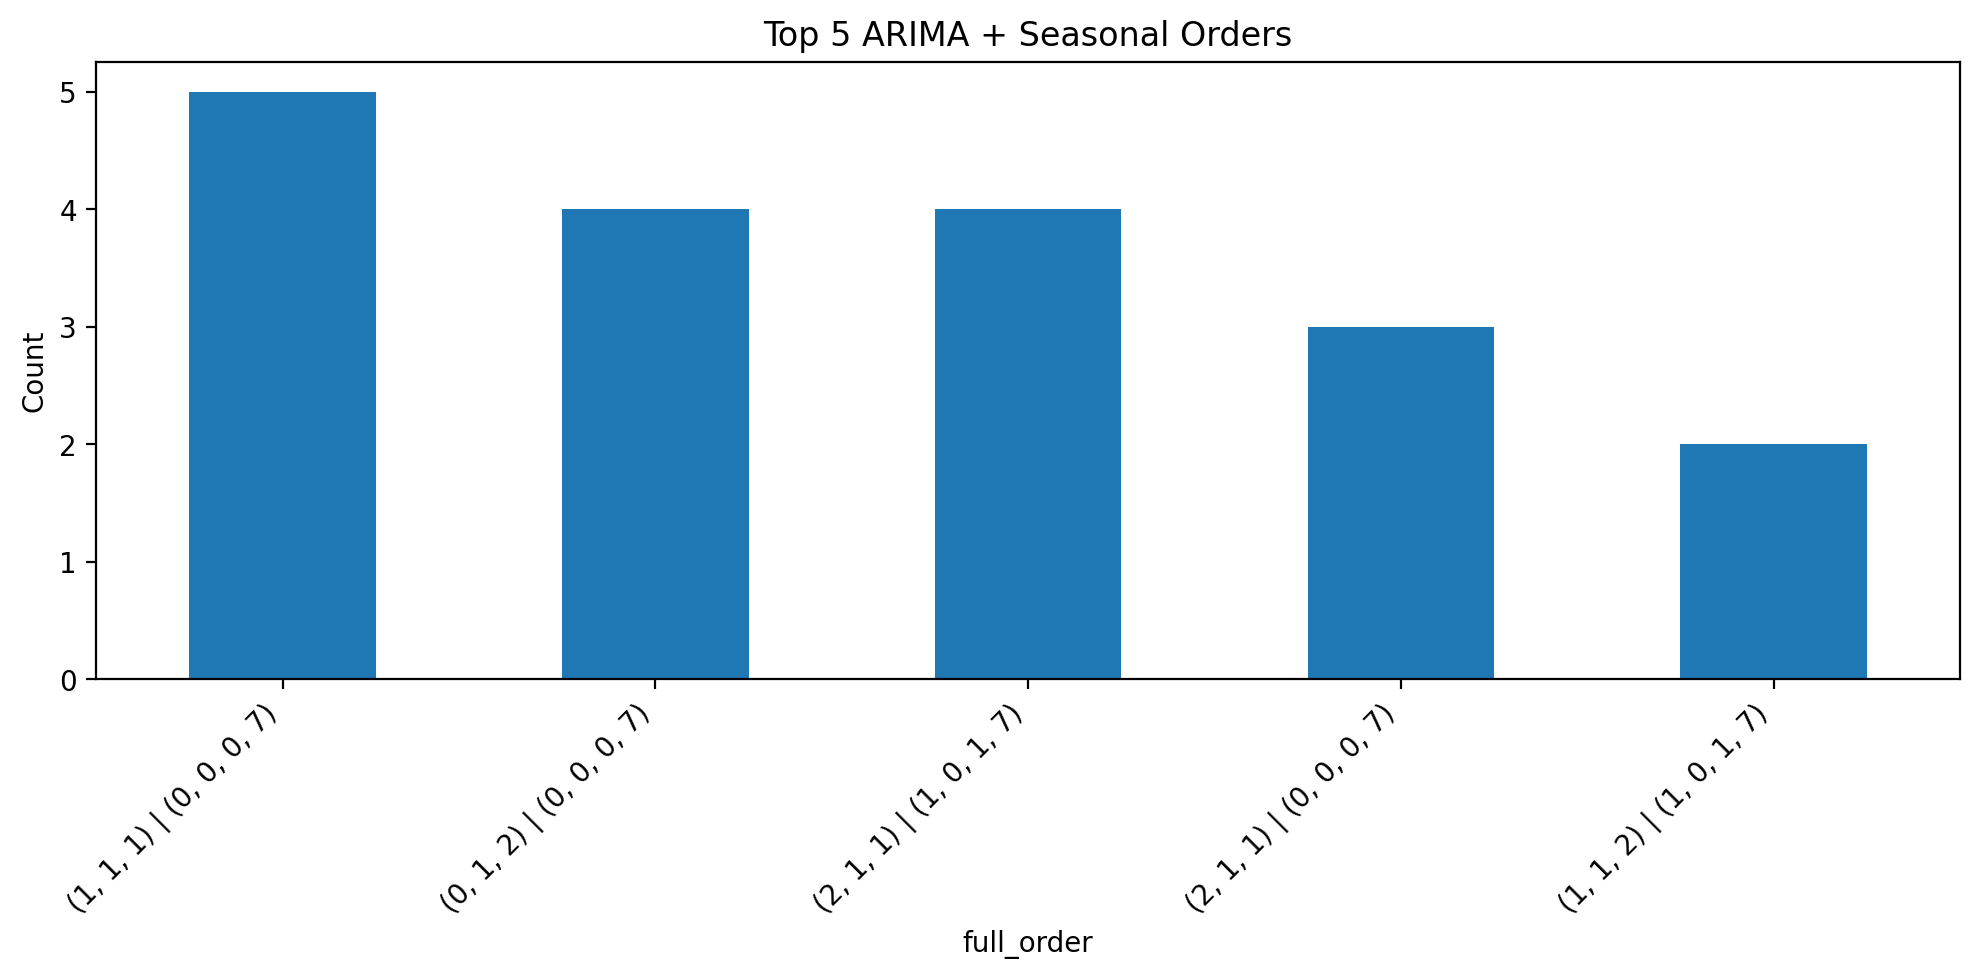
\includegraphics[width=0.9\linewidth]{figures/arima_seasonal_pre_order.png}
        \caption{ARIMA order frequency for seasonal cell}s
        \label{fig:arima_seasonal_pre_order}
    \end{subfigure}

    \vspace{0.5cm}

    \begin{subfigure}[b]{0.9\linewidth}
        \centering
        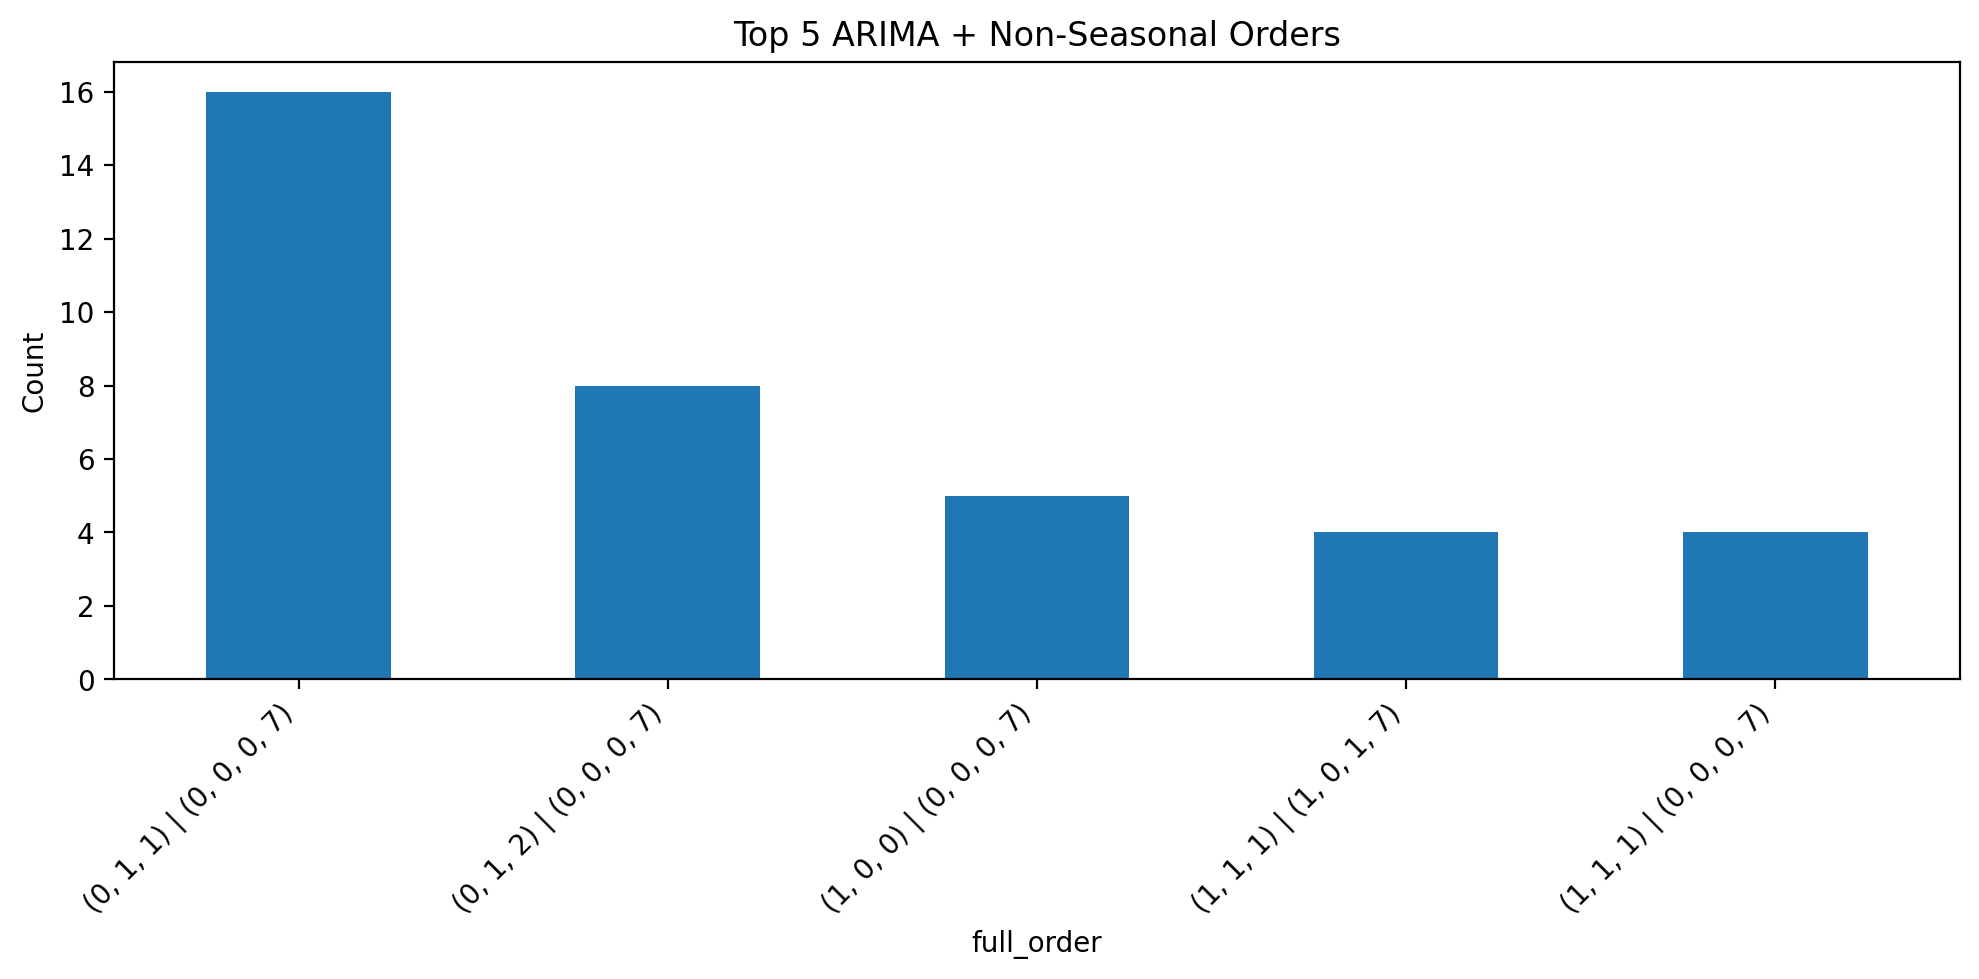
\includegraphics[width=0.9\linewidth]{figures/arima_non_seasonal_pre_order.png}
        \caption{ARIMA order frequency for non-seasonal cell}
        \label{fig:arima_non_seasonal_pre_order}
    \end{subfigure}
    
    \begin{subfigure}[b]{0.9\linewidth}
        \centering
        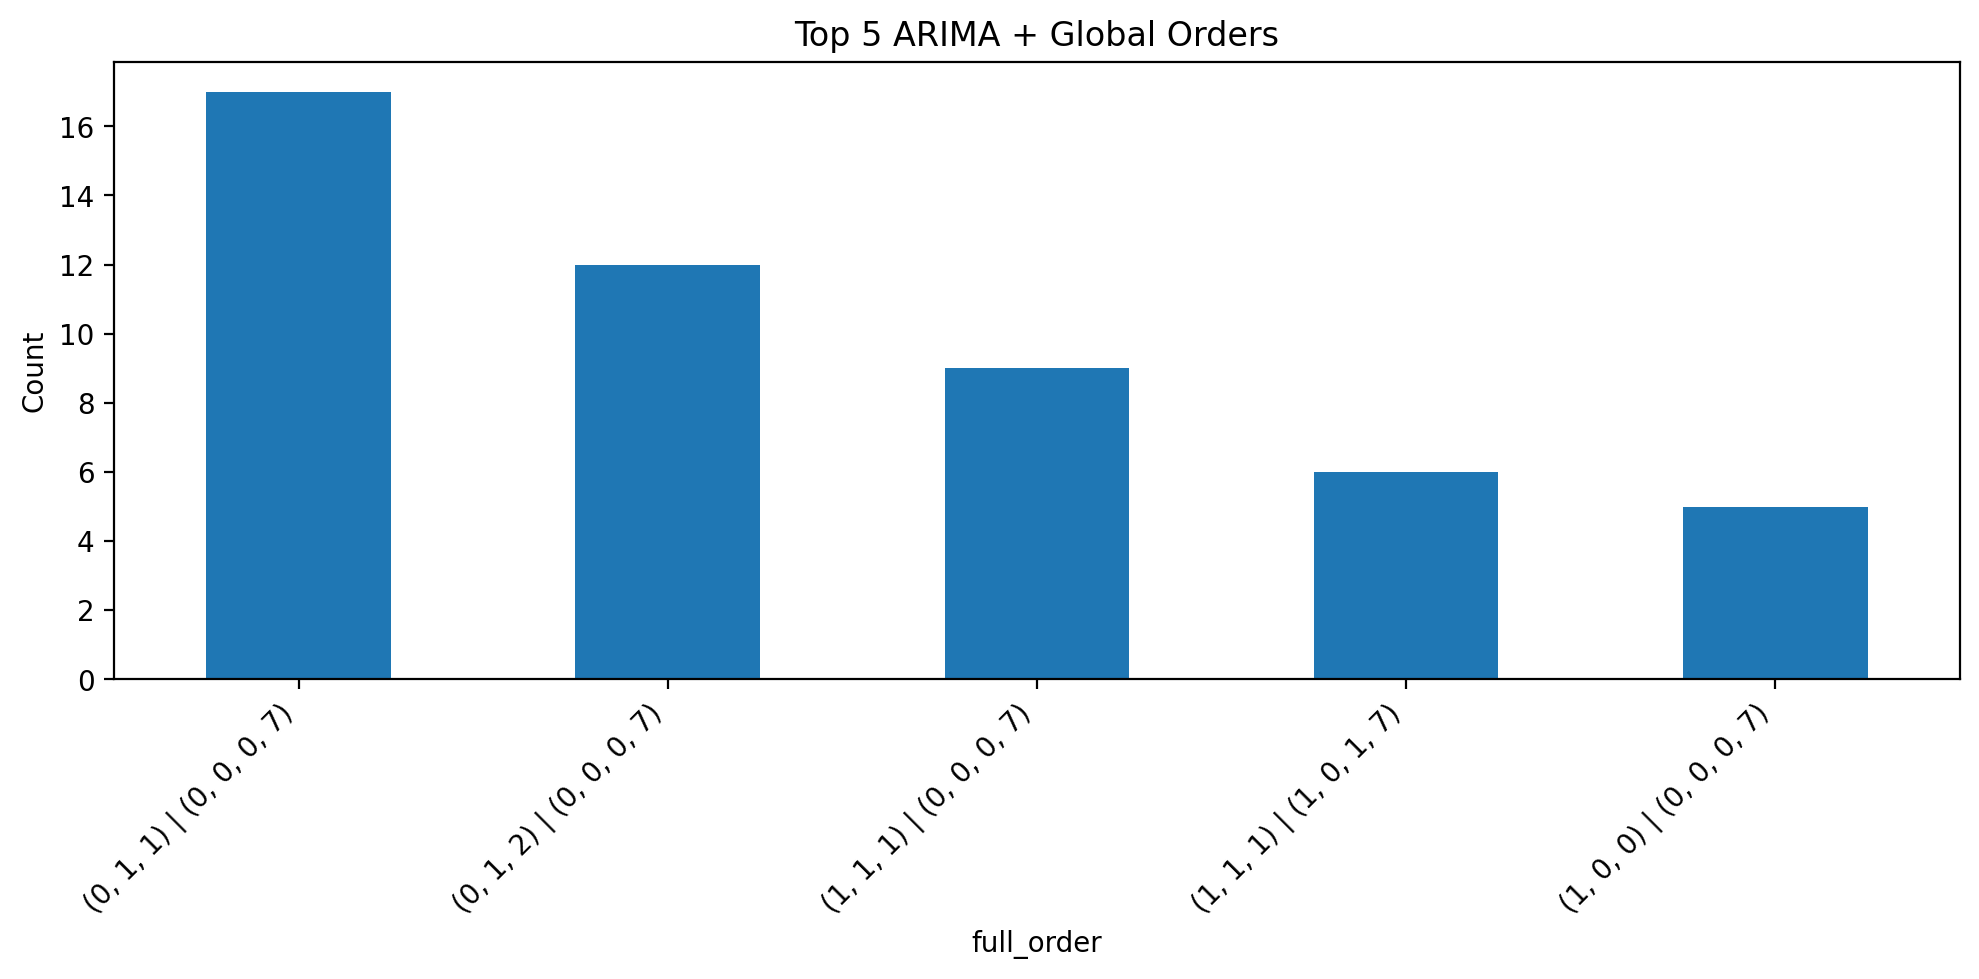
\includegraphics[width=0.9\linewidth]{figures/arima_global_pre_order.png}
        \caption{ARIMA order frequency for all cells}
        \label{fig:arima_global_pre_order}
    \end{subfigure}
    
    \caption{Arima order before feature selection}
    \label{fig:pre_order_arima}
\end{figure}

Figure~\ref{fig:pre_order_arima} shows the frequency of the ARIMA orders selected by the auto-ARIMA procedure across all seasonal cell time series. \\

For the seasonal setting, the most frequently selected configuration was ARIMA$(1,1,1)(0,0,0,7)$. This indicates that first-order differencing was consistently required, while the dominant structure was captured through short-term autoregressive and moving-average components. \\

For the non-seasonal setting, the dominant configuration was ARIMA$(0,1,1)(0,0,0, 7)$. Compared to the seasonal case, the autoregressive component disappeared, suggesting weaker temporal dependence in the non-seasonal cells. However, first-order differencing, the moving-average and seasonal components remained consistently selected across both groups. \\

\subsubsection{Feature selection}
To evaluate the impact of exogenous variables on forecasting performance, a forward feature selection approach was used. The goal was to iteratively build a feature set that minimizes the mean squared error (MSE) across all time series (cells). \\

Table~\ref{tab:tested_features} shows the set of candidate features evaluated during the selection process.

\begin{table}[htbp]
\centering
\caption{Candidate features evaluated during feature selection}
\label{tab:tested_features}

\begin{tabular}{ll}
\toprule
\textbf{Feature} & \textbf{Description} \\
\midrule
month & Month of the year \\
dayofweek & Day of the week \\
is\_weekend & Weekend indicator variable \\
holiday & Public holiday indicator \\
lag1 & Previous day traffic value \\
lag7 & Traffic value from 7 days earlier \\
roll\_mean\_7 & Rolling 7-day mean \\
roll\_mean\_14 & Rolling 14-day mean \\
roll\_std\_7 & Rolling 7-day standard deviation \\
roll\_std\_14 & Rolling 14-day standard deviation \\
roll\_min\_7 & Rolling 7-day minimum \\
roll\_max\_7 & Rolling 7-day maximum \\
lag\_diff\_1\_7 & Difference between lag-1 and lag-7 \\
\bottomrule
\end{tabular}
\end{table}

To evaluate the impact of exogenous variables on forecasting performance, a forward feature selection approach is applied. The method starts with an empty feature set and iteratively adds the feature that yields the largest reduction in average test mean squared error (MSE) across all time series. Candidate features include calendar variables, lag-based features, rolling statistics, and differenced features. The process continues until no further improvement is observed, as shown in Algorithm \ref{alg:algo_1}.\\

\begin{algorithm}[H]\caption{Forward Feature Selection for ARIMA with Exogenous features}
\begin{algorithmic}[1]

\STATE Initialize selected feature set $S \leftarrow \emptyset$
\STATE Initialize remaining features $R \leftarrow \{f_1, f_2, ..., f_n\}$
\STATE Set best error $E_{best} \leftarrow \infty$

\WHILE{$R \neq \emptyset$}
    \STATE $f^* \leftarrow \emptyset$
    \STATE $E^* \leftarrow E_{best}$

    \FOR{each feature $f \in R$}
        \STATE Train ARIMA models with feature set $S \cup \{f\}$ across all series
        \STATE Evaluate mean test error $E_f$
        
        \IF{$E_f < E^*$}
            \STATE $E^* \leftarrow E_f$
            \STATE $f^* \leftarrow f$
        \ENDIF
    \ENDFOR

    \IF{$f^* \neq \emptyset$}
        \STATE Add $f^*$ to $S$
        \STATE Remove $f^*$ from $R$
        \STATE Update $E_{best} \leftarrow E^*$
    \ELSE
        \STATE Stop
    \ENDIF

\ENDWHILE

\end{algorithmic}
\label{alg:algo_1}
\end{algorithm}

The forward selection procedure is applied separately to three model configurations: seasonal cells, non-seasonal cells, and the full dataset. Each configuration follows the same evaluation protocol, where features are added sequentially based on their impact on validation RMSE. The final selected feature set for each configuration is determined when no additional feature yields further improvement. \\
\begin{table}[htbp]
\centering
\caption{Feature selection results across seasonal, non-seasonal, and all-cell models}
\label{tab:feature_selection_all}

\begin{tabular}{lcc}
\toprule
\textbf{Model Type} & \textbf{Selected Features (final step)} & \textbf{RMSE} \\
\midrule
Seasonal cells & roll\_mean\_7, roll\_max\_7 & 1.62 \\
Non-seasonal cells & roll\_min\_7, lag\_1, is\_weekend & 1.71 \\
All cells & roll\_min\_7, lag\_1, lag\_diff\_1\_7 & 1.66 \\
\bottomrule
\end{tabular}
\end{table}

Feature selection results show strong overlap between the non-seasonal and all-cell configurations, which converge to the same optimal feature set. In contrast, seasonal cells rely more on short-term aggregated statistics such as rolling means and maxima, while non-seasonal cells benefit from lag-based and difference features that capture local temporal changes. \\

Across all configurations, performance improvements are primarily driven by short-term dependency features (lag-1 and lag-difference), suggesting that recent history dominates predictive power. Seasonal structure contributes less to overall error reduction, indicating weak or inconsistent periodicity across most cells. \\


\subsubsection{Post feature selection order refinement}

After feature selection, the top ARIMA orders identified during the baseline stage were re-evaluated using the selected exogenous variables. Each configuration was refitted and tested on the held-out dataset, and performance was compared to the feature-selection baseline.

\begin{figure}[H]
	\centering
	
	\begin{subfigure}[b]{0.9\linewidth}
		\centering
		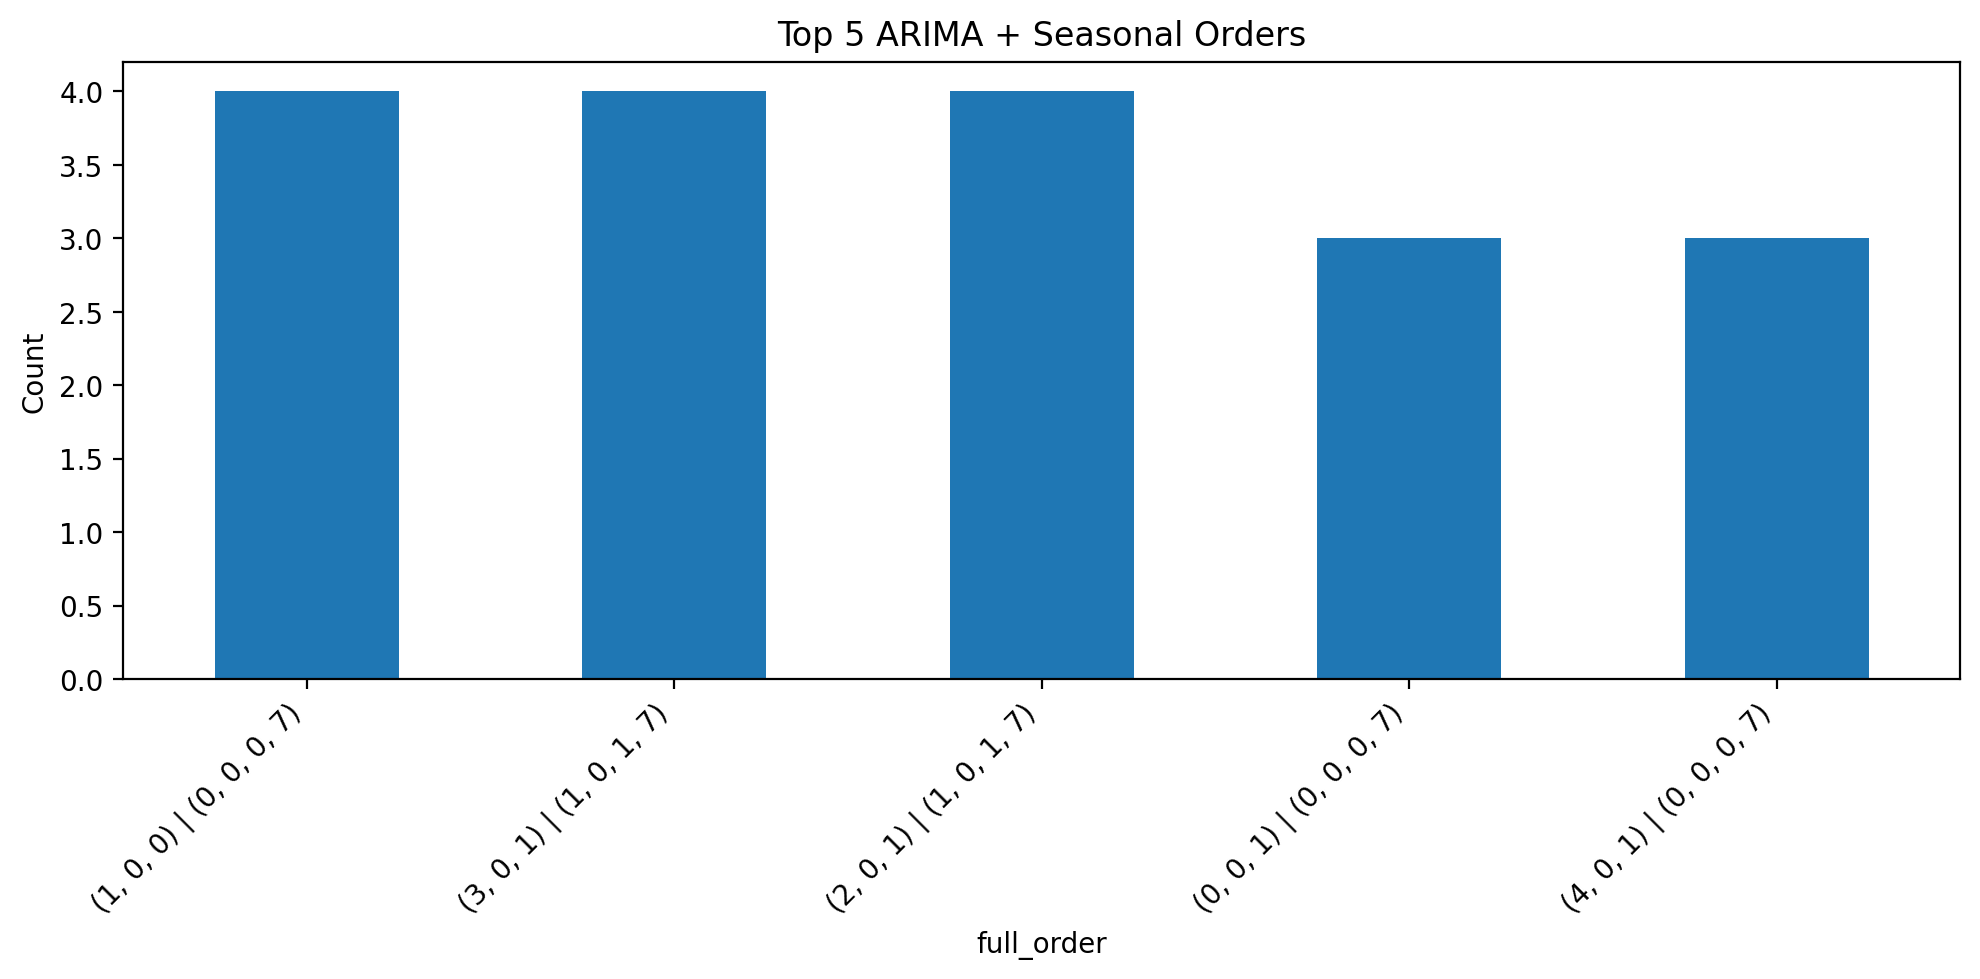
\includegraphics[width=0.9\linewidth]{figures/arima_post_seasonal_order_2.png}
		\caption{ARIMA order frequency for seasonal cells}
		\label{fig:arima_seasonal_post_order}
	\end{subfigure}
	
	\vspace{0.5cm}
	
	\begin{subfigure}[b]{0.9\linewidth}
		\centering
		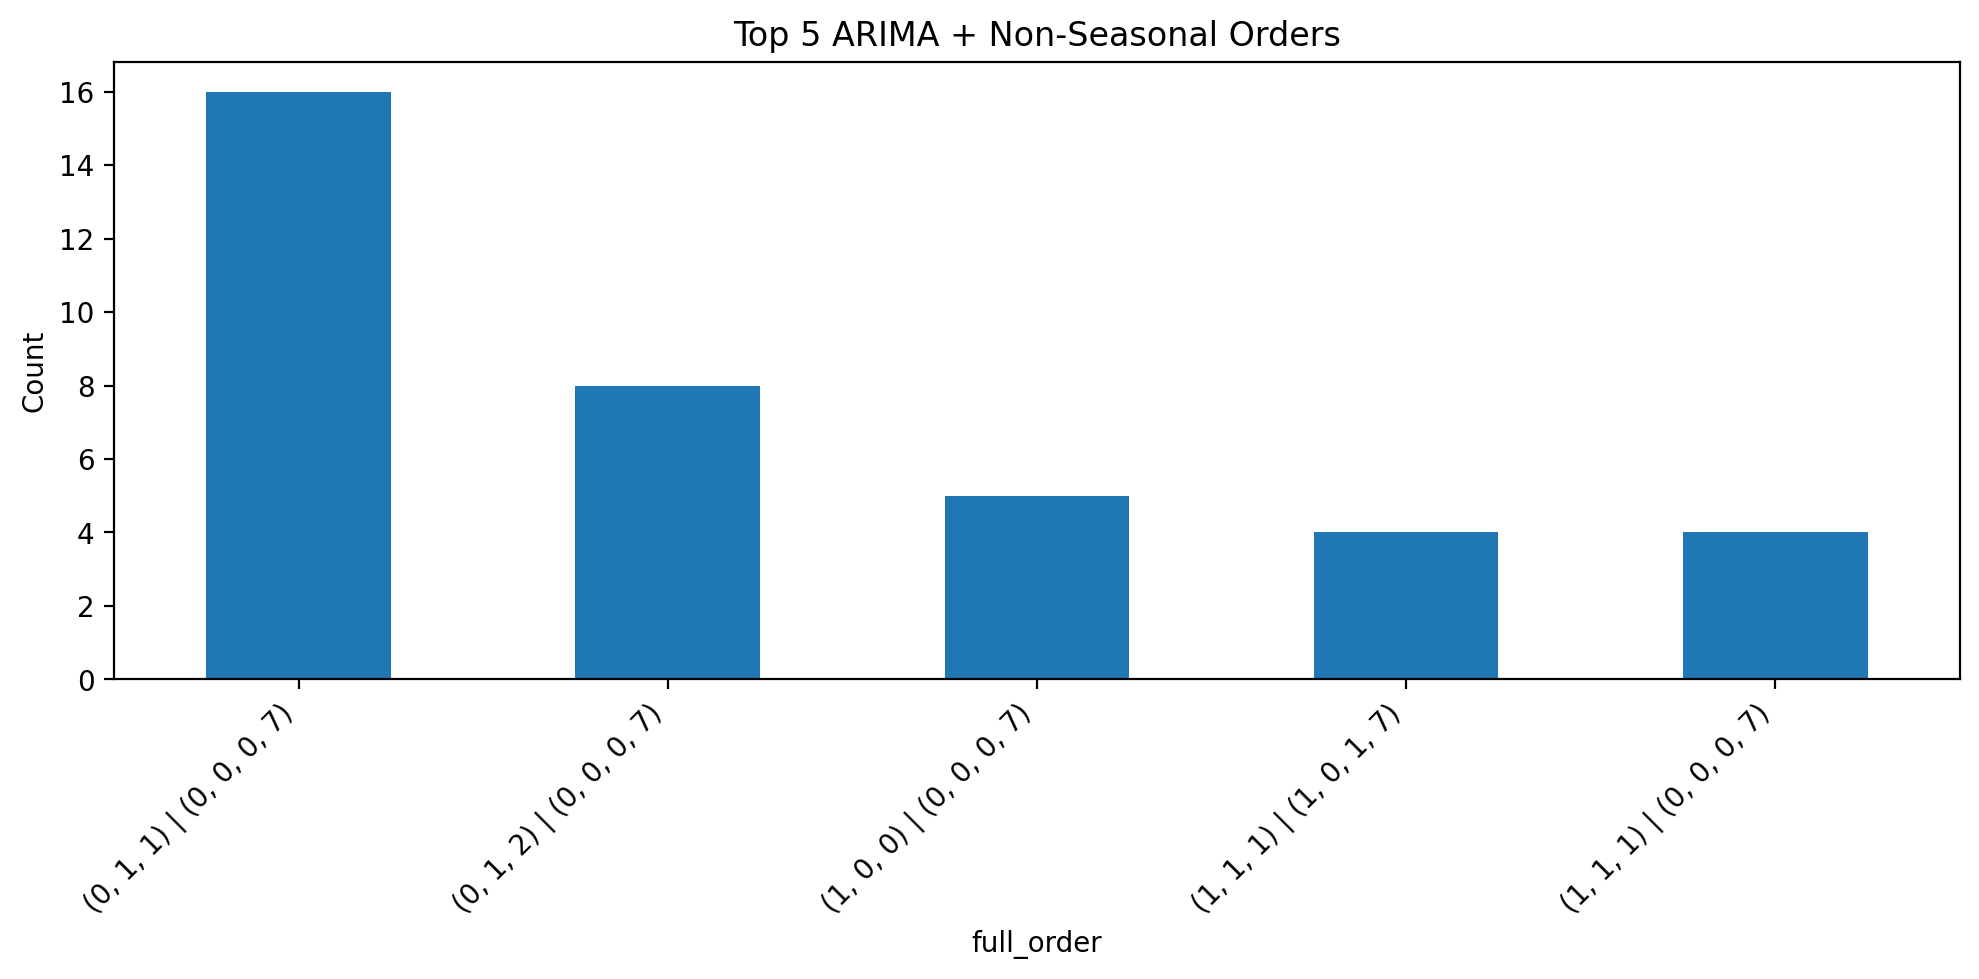
\includegraphics[width=0.9\linewidth]{figures/arima_non_seasonal_pre_order_2.png}
		\caption{ARIMA order frequency for non-seasonal cells}
		\label{fig:arima_non_seasonal_post_order}
	\end{subfigure}
	
	\begin{subfigure}[b]{0.9\linewidth}
		\centering
		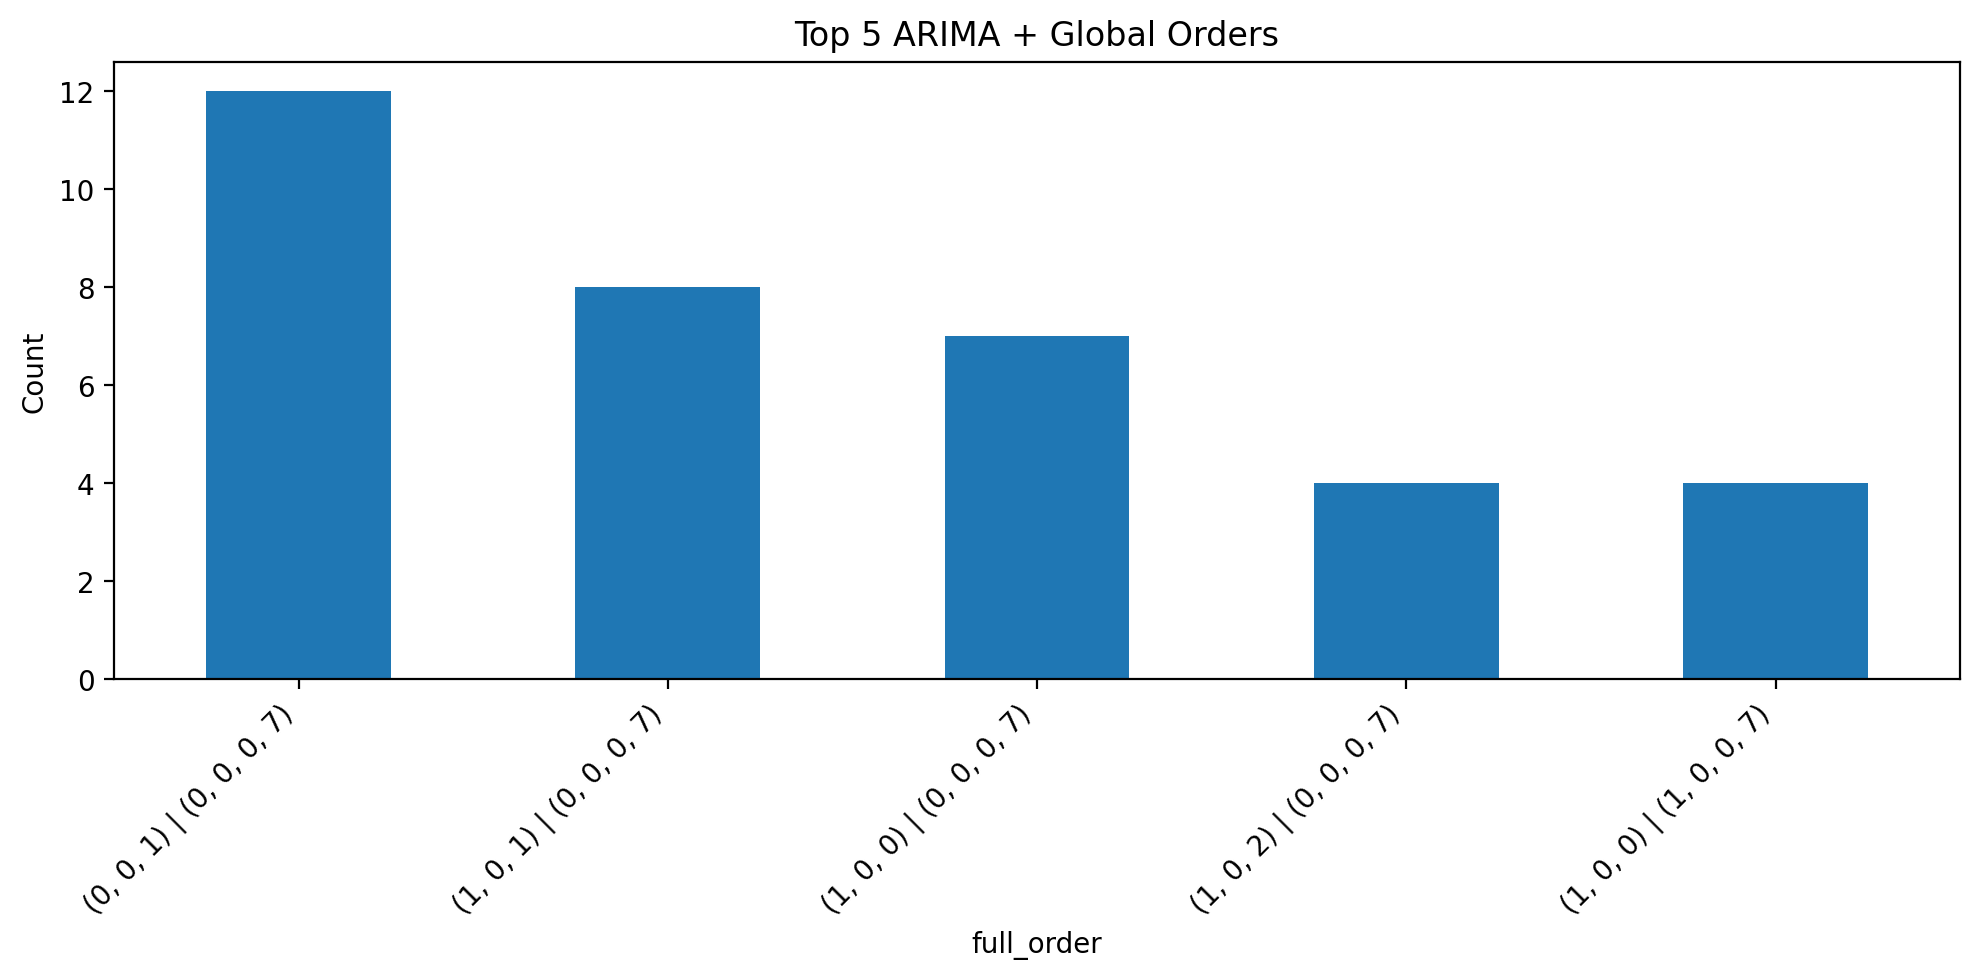
\includegraphics[width=0.9\linewidth]{figures/arima_global_post_order.png}
		\caption{ARIMA order frequency for all cells}
		\label{fig:arima_global_post_order}
	\end{subfigure}
	
	\caption{ARIMA order selection after feature engineering}
	\label{fig:arima_post_orders}
\end{figure}

The results show only limited changes after feature selection. For seasonal cells, a slightly different configuration ARIMA$(0,0,1)(0,0,0,7)$ achieved the best performance with an RMSE of 1.51. For non-seasonal cells and all cells, the original configuration ARIMA$(0,1,1)(0,0,0,7)$ remained optimal.

\begin{table}[htbp]
	\centering
	\caption{Post feature selection ARIMA performance comparison}
	\label{tab:arima_post_results}
	
	\begin{tabular}{lcc}
		\toprule
		\textbf{Model Type} & \textbf{Best Order} & \textbf{RMSE} \\
		\midrule
		Seasonal cells & $(0,0,1)(0,0,0,7)$ & 1.5139 \\
		Non-seasonal cells & $(0,1,1)(0,0,0,7)$ & 1.7102 \\
		All cells (global) & $(0,1,1)(0,0,0,7)$t & 1.6600 \\
		\bottomrule
	\end{tabular}
\end{table}

Overall, the results suggest that both feature engineering and model order selection contribute to forecasting performance. Feature selection provides the main improvement, while re-tuning the ARIMA order after feature selection yields only marginal additional gains. \\

For seasonal cells, a small but consistent improvement is observed after adjusting the ARIMA order, reducing the RMSE from the feature-selection baseline. For non-seasonal and global models, changes in ARIMA order do not lead to meaningful improvements. \\

This indicates that exogenous features carry most of the predictive signal, while ARIMA order tuning provides secondary refinement in certain cases rather than large performance shifts. \\

\begin{figure}[H]
	\centering
	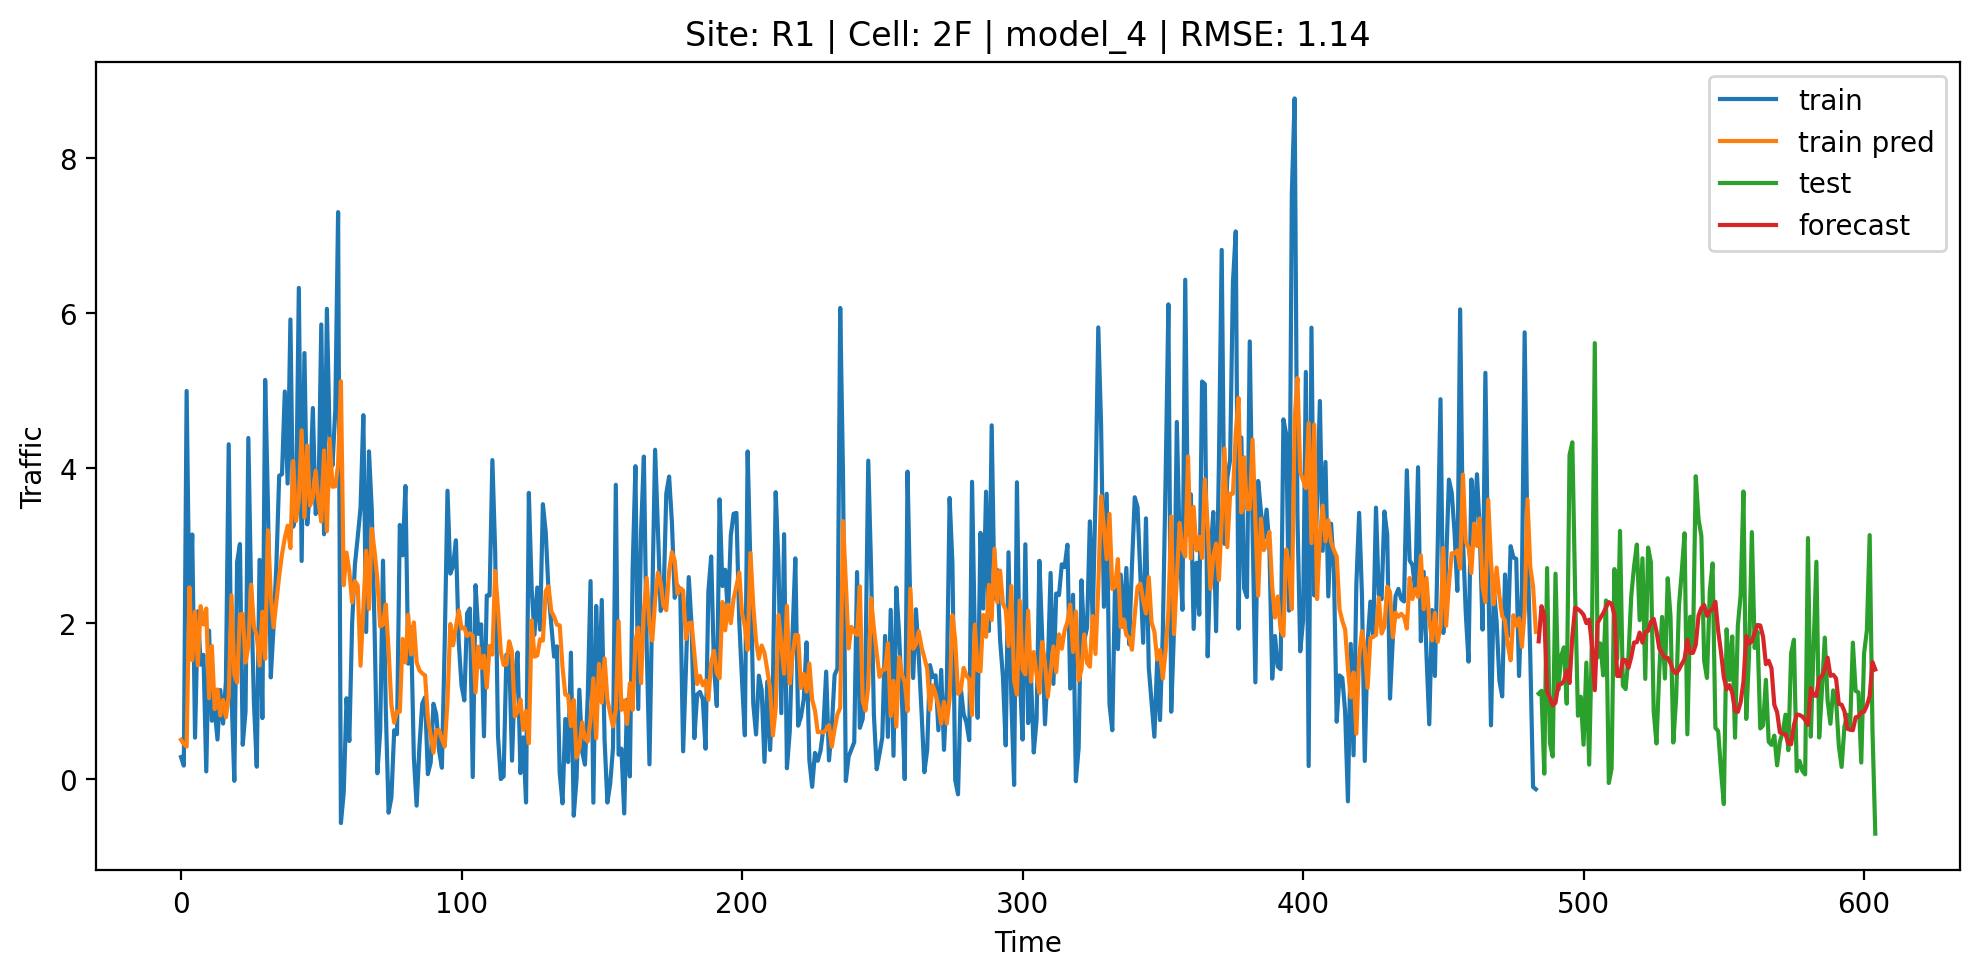
\includegraphics[width=\linewidth]{figures/arima_pred.png}
	\caption{Seasonal Arima Fitting and Prediction on R1 2F}
	\label{fig:arima_prediction}
\end{figure}

To better understand model behaviour, Figure~\ref{fig:arima_prediction} shows the fitted values on the training data and the predictions on the held-out test set for a representative cell (R1, 2F). \\







\subsection{Ordinary Least Squares}
Ordinary Least Squares (OLS) is a linear regression method that estimates parameters by minimizing the sum of squared errors between observed values and predictions.

In the simplest case with one feature, OLS fits a line of the form:
\[
y = \beta_0 + \beta_1 x
\]
where $\beta_0$ is the intercept and $\beta_1$ is the slope. These are chosen to minimize:
\[
\min_{\beta_0, \beta_1} \sum_{i=1}^{n} (y_i - (\beta_0 + \beta_1 x_i))^2
\]

Unlike ARIMA, which models temporal dependence using past values of the time series, OLS does not assume any time structure. Each observation is treated as independent.

With multiple features, OLS generalizes to:
\[
y = \beta_0 + \beta_1 x_1 + \beta_2 x_2 + \dots + \beta_p x_p
\]

or in matrix form:
\[
\mathbf{y} = \mathbf{X}\boldsymbol{\beta} + \boldsymbol{\epsilon}
\]

Here, $\mathbf{X}$ is the feature matrix, $\boldsymbol{\beta}$ is the vector of learned coefficients, and $\boldsymbol{\epsilon}$ is the error term. \\

Each feature contributes additively to the prediction through its own weight, along with a single shared intercept. This allows OLS to incorporate engineered inputs such as lagged values, rolling statistics, or external variables, but it does not explicitly model time dynamics.

\subsubsection{Feature selection}

The same forward feature selection procedure used for the SARIMAX models (Algorithm~\ref{alg:algo_1}) was applied to the OLS model. The candidate feature pool, evaluation metric, and stopping criterion were kept identical to ensure a fair comparison between the two approaches.

At each iteration, an OLS model was fitted using the current selected feature set and one additional candidate feature. The feature producing the largest reduction in validation RMSE was retained. The process continued until no further improvement in performance was observed.

\subsubsection{results}
The results for the 3 data grops were as follows

\subsection{XGboost}
Unlike the statistical models presented in the previous sections, XGBoost (Extreme Gradient Boosting) is a machine learning method that makes no parametric assumptions about the underlying data generating process. Where ARIMA models temporal dependence explicitly through autoregressive and moving average components, and OLS assumes a fixed linear relationship between features and the target, XGBoost learns complex non-linear interactions directly from data by sequentially fitting an ensemble of decision trees, each correcting the residual errors of the previous one. \\

A key practical distinction from the models presented earlier is that XGBoost is data-hungry. Cell-specific models, as applied in the ARIMA and OLS sections, operate on a single time series at a time and are therefore well suited to small, isolated datasets. XGBoost however benefits substantially from volume and diversity of training examples. For this reason, all cells across all sites are pooled into a single dataset, allowing the model to learn shared patterns across the entire network simultaneously. \\
This global training approach also changes how cell identity is handled. Rather than fitting a separate model per cell, the cell and site are included as encoded input features, allowing the model to naturally condition its predictions on cell-specific behavior where such structure exists in the data. If a particular cell or site exhibits a distinct traffic pattern, the model will capture this through its learned splits without requiring explicit pre-classification into seasonal and non-seasonal groups as was necessary for the statistical approaches. \\

\subsubsection{Decision tree}
A decision tree works by repeatedly splitting the data based on a single feature and threshold at a time. There is no linearity involved — the model does not assign weights to features or assume any functional form. It simply partitions the feature space into regions, and every observation that falls into the same region receives the same prediction. A single tree of this kind is a very crude approximation, and in practice a single tree tends to overfit easily. \\

Random forests address this by training many trees independently on random subsets of the data and features, a technique known as bootstrapping, and averaging their predictions. This reduces variance and makes the model considerably more robust than any individual tree. \\
XGBoost follows the same principle of combining many trees, but rather than training them independently, it builds them sequentially. Each new tree is fitted to the errors left by all previous trees, so the ensemble improves iteratively rather than by averaging. The final prediction is the sum of all trees: 
\[
\hat{y}_i = \sum_{k=1}^{K} f_k(\mathbf{x}_i)
\]
This approach is known as gradient boosting, and XGBoost is a highly optimised implementation of it that has become one of the most widely used models in applied machine learning. \\

\subsubsection{Implementation}
Since XGBoost processes one observation at a time and has no built-in notion of time or sequential order, it cannot look back at past values the way ARIMA does. This makes feature engineering particularly important. All temporal context that the model needs to understand historical behaviour must be explicitly constructed and provided as input features. With this in mind, the feature set was designed to capture both temporal patterns and cell-specific characteristics, and can be grouped into the following categories. \\

\textbf{Raw network metrics} were included directly from the dataset, covering downlink and uplink data volumes, PRB utilisation, active UEs, throughput, and SINR measurements. These provide the model with direct signal about the current network state. \\

\textbf{Lag features} capture historical values of the target at fixed time offsets: 1, 8, 24, 168, and 720 hours back. These allow the model to condition its prediction on recent observations as well as patterns from the same hour yesterday, the same day last week, and the same period last month.
\textbf{Rolling statistics} were computed across a wide range of windows: 3, 6, 12, 24, 48, 168, 336, 720, and 2160 hours. For each window, the mean, maximum, minimum, and standard deviation were included. This gives the model a rich view of both short-term fluctuations and long-term trends. \\

\textbf{Calendar features} were one-hot encoded to allow the model to learn non-linear patterns tied to time. This includes the hour of the day (0--23), day of the week (0--6), and month of the year (1--12), as well as binary indicators for weekends and public holidays. \\
\textbf{Cell and technology features} were included to allow the model to differentiate between cells. The site group and technology generation (4G/5G) were one-hot encoded, along with the frequency band, covering LTE800, LTE1800, LTE2600, NR700, and NR3500. A binary seasonal indicator was also included based on the pre-classification described in earlier sections.\\

In total this results in \textbf{107 input features} per observation. \\

\subsubsection{XG Boost Results}

The model was trained with 200 trees, a learning rate of 0.05, and a maximum tree depth of 4. The data was split chronologically with 80 percent used for training and 20 percent held out for testing. The final model achieved an RMSE of 1.70 on the test set. \\

\begin{figure}[H]
	\centering
	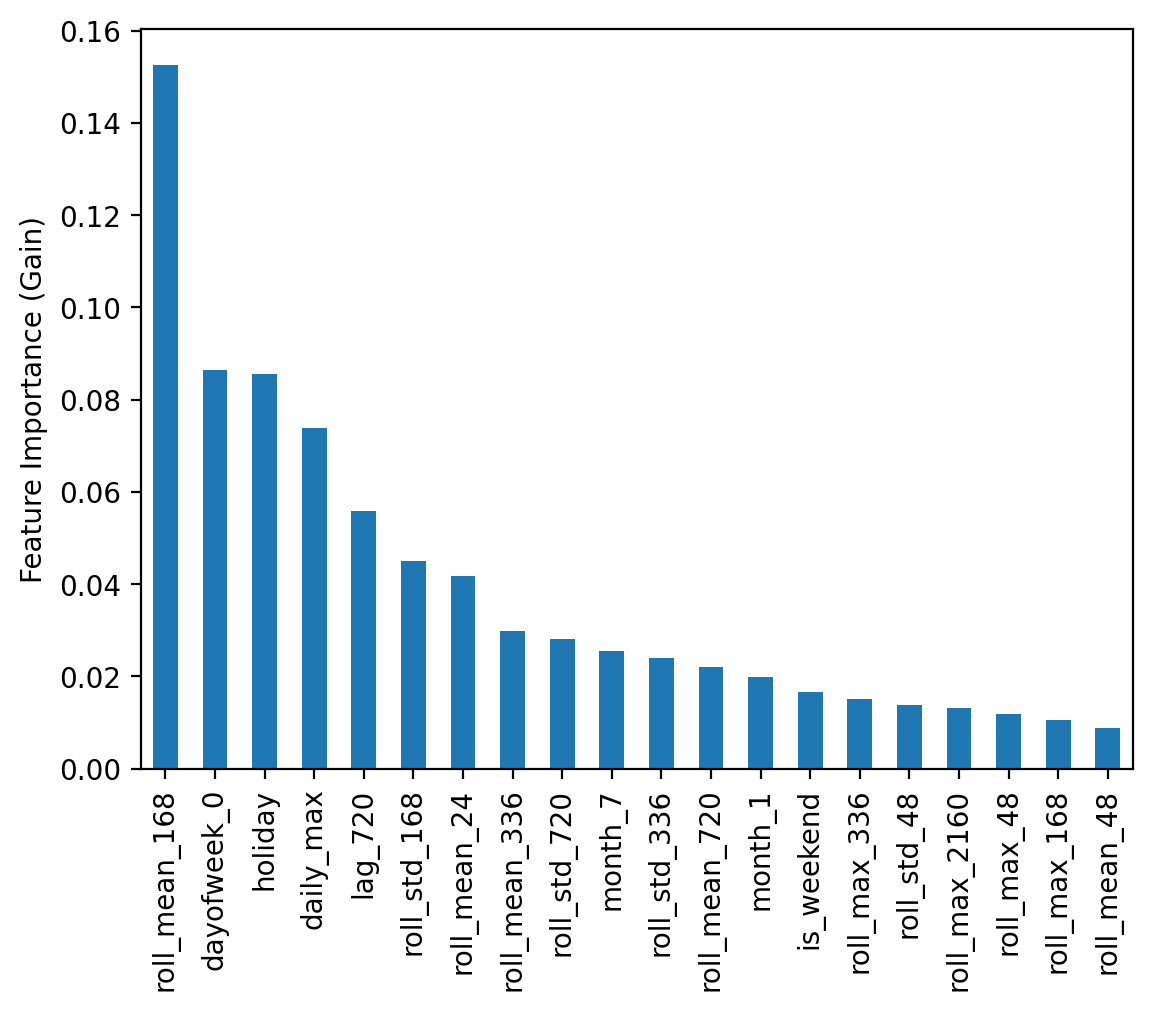
\includegraphics[width=\linewidth]{figures/feature_importance_xg.png}
	\caption{XG Boost feature importance}
	\label{fig:xg_feature_importance}
\end{figure}

Figure~\ref{fig:xg_feature_importance} shows the feature importances assigned by the model, measured by gain, which reflects how much each feature reduces the prediction error on average across all splits where it is used. The most influential feature was \texttt{roll\_mean\_168}, the rolling mean over the past week, with a gain of 0.15. This suggests that the average traffic level over the previous seven days is the single strongest predictor of the next day daily maximum. Calendar features also rank highly, with \texttt{dayofweek\_0} and \texttt{holiday} achieving gains of 0.09 and 0.09 respectively, indicating that the model has picked up on weekly rhythms and public holiday effects. Other notable features include \texttt{daily\_max} at 0.07, \texttt{lag\_720} at 0.06, and \texttt{roll\_std\_168} at 0.04, reinforcing that medium to long-term historical behaviour dominates the predictions. \\

\begin{figure}[H]
	\centering
	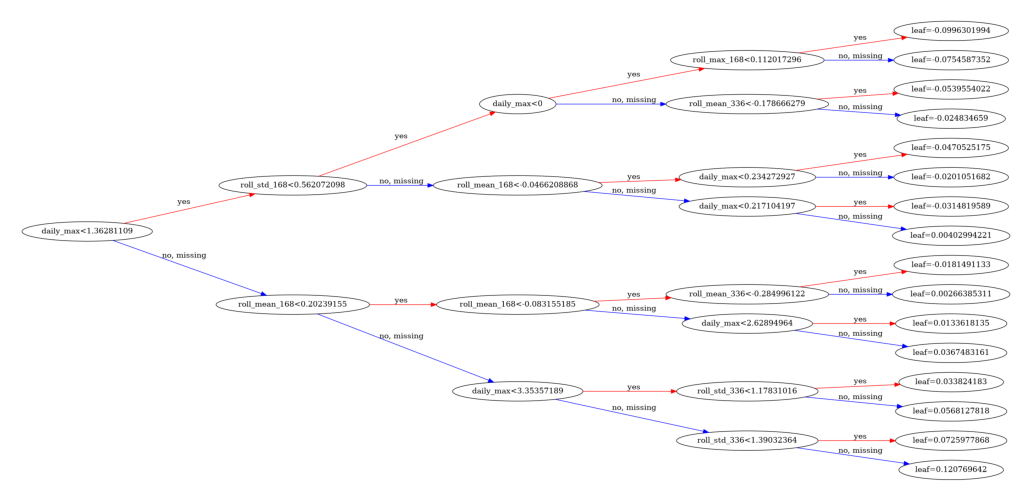
\includegraphics[width=\linewidth]{figures/xg_tree.png}
	\caption{A single tree from XG model}
	\label{fig:xg_tree}
\end{figure}

Figure~\ref{fig:xg_tree} visualises a single tree from the ensemble. At each internal node the tree makes a binary decision based on a threshold for a given feature, routing each observation either left or right until it reaches a leaf node where a prediction is made. With a maximum depth of 4, the tree can make at most 4 consecutive splits, resulting in up to 16 leaf nodes each outputting a distinct predicted value. It is worth noting that this is just one of the 200 trees that make up the final model, and on its own it is a very coarse approximation. \\

\begin{figure}[H]
	\centering
	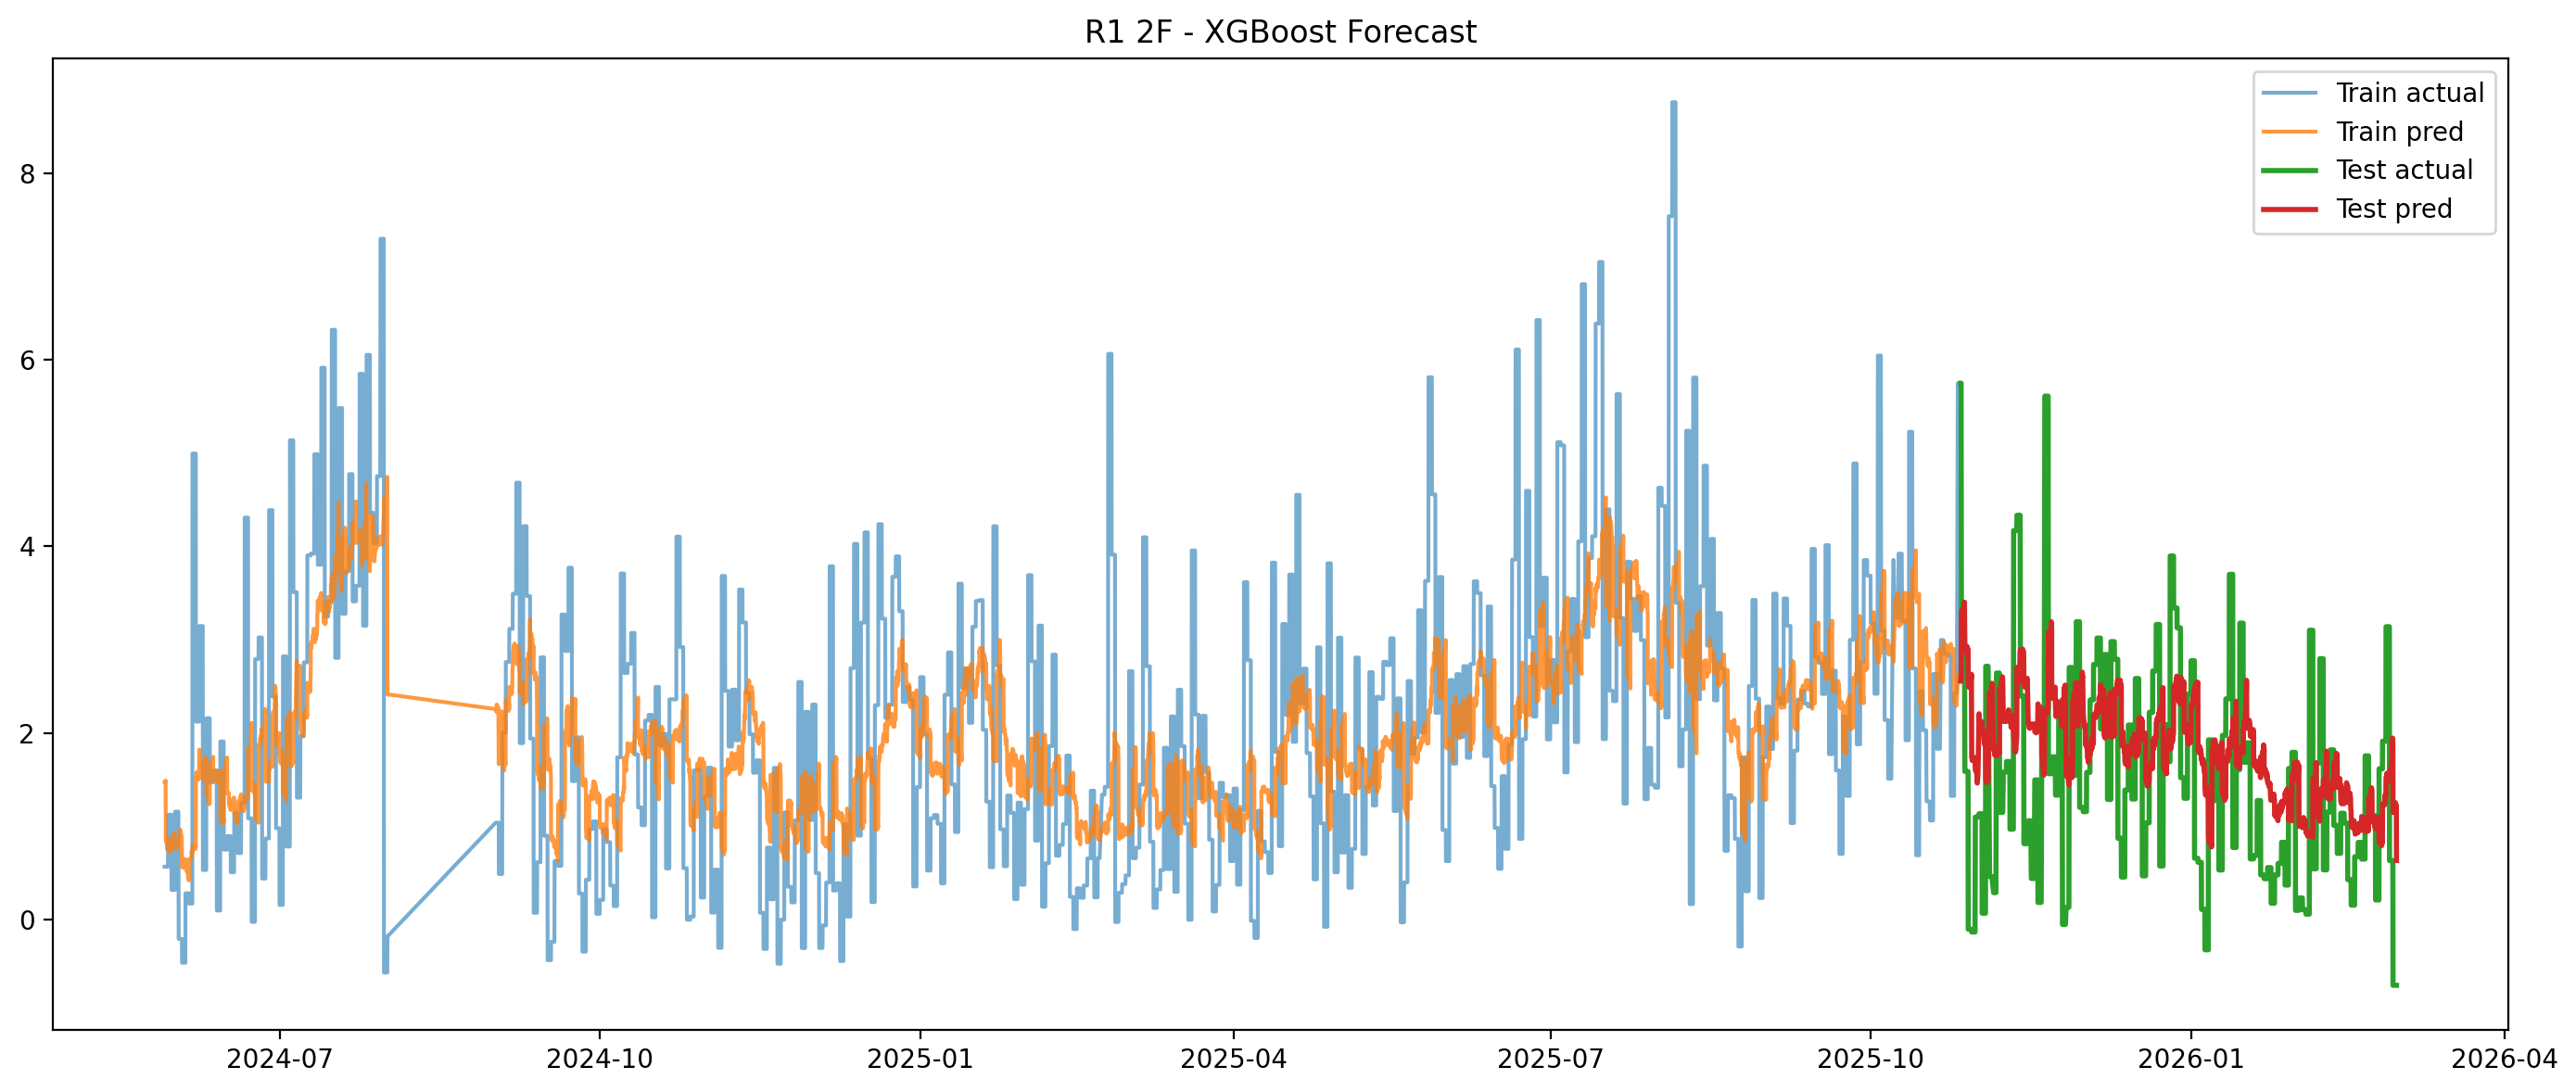
\includegraphics[width=\linewidth]{figures/xg_boost_prediction.png}
	\caption{Prediction vs Actual, xg boost on site R1 cell 2F}
	\label{fig:xg_boost_prediction}
\end{figure}

Figure~\ref{fig:xg_boost_prediction} shows the predicted versus actual daily maximum for site R1, cell 2F. The model captures the general trend and seasonal fluctuations reasonably well, though some peaks are underestimated, which is a common characteristic of tree based models that predict based on previously seen value ranges. \\










 
 